Dada la separación en cascada realizada en la sección 1 para $H(s) = H_1(s)\cdot H_2(s)$, donde cada H es de la forma:
$$
    H_i = \frac{K_i s^2}{s^2 + b_i \cdot s + c_i}
$$
Teniendo en cuenta que el siguiente circuito
\begin{figure}[H]
    \centering
    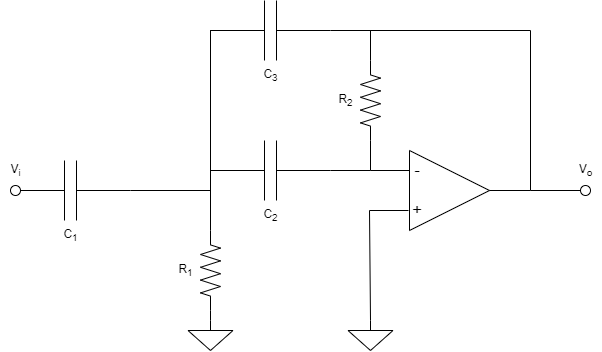
\includegraphics[width=1\textwidth]{resources/Filtro.png}
    \caption{Circuito pasa altos con retroalimentación múltiple}
\end{figure}

posee una transferencia definida
$$
    H^{*}(s) = \frac{-\frac{C_1}{C_3}s^2}{s^2+\frac{C_1+C_2+C_3}{R_2C_2C_3}s+\frac{1}{R_1R_2C_2C_3}}
$$
\vskip0.5cm

Entonces, ambas transferencias $H_1$ y $H_2$ podrán ser implementadas a partir de este circuito. Quedando entonces el siguiente filtro:
\begin{figure}[H]
    \centering
    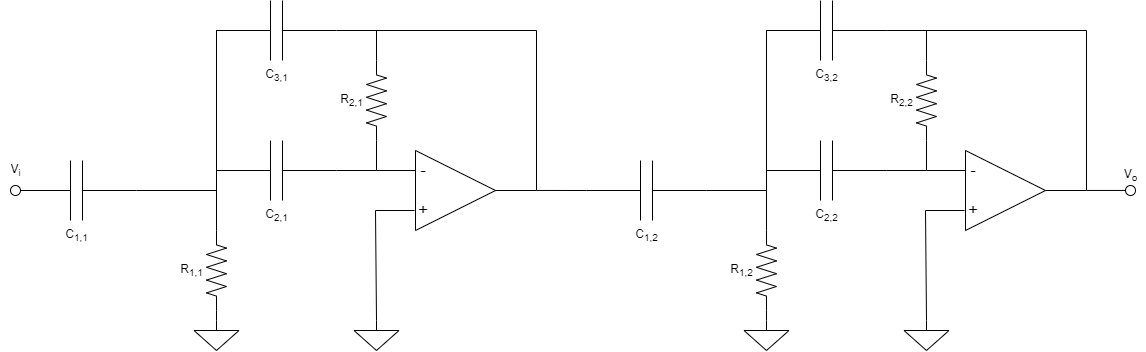
\includegraphics[width=1\textwidth]{resources/FiltroCompleto.png}
    \caption{Implementación del filtro}
\end{figure}

Siendo finalmente la transferencia:

$$
    H(s) = \frac
            {\frac{C_{1,1}C_{1,2}}{C_{3,1}C_{3,2}}s^4}
            {(s^2 +\frac{C_{1,1}+C_{2,1}+C_{3,1}}{R_{2,1}C_{2,1}C_{3,1}}s+\frac{1}{R_{1,1}R_{2,1}C_{2,1}C_{3,1}}) (s^2 +\frac{C_{1,2}+C_{2,2}+C_{3,2}}{R_{2,2}C_{2,2}C_{3,2}}s+\frac{1}{R_{1,2}R_{2,2}C_{2,2}C_{3,2}})}
$$